%%%%%%%%%%%%%%%%%%%%%%%%%%%%%%%%%%%%%%%%%
% Programming/Coding Assignment
% LaTeX Template
%
% This template has been downloaded from:
% http://www.latextemplates.com
%
% Original author:
% Ted Pavlic (http://www.tedpavlic.com)
%
% Note:
% The \lipsum[#] commands throughout this template generate dummy text
% to fill the template out. These commands should all be removed when 
% writing assignment content.
%
% This template uses a Perl script as an example snippet of code, most other
% languages are also usable. Configure them in the "CODE INCLUSION 
% CONFIGURATION" section.
%
%%%%%%%%%%%%%%%%%%%%%%%%%%%%%%%%%%%%%%%%%

%----------------------------------------------------------------------------------------
%	PACKAGES AND OTHER DOCUMENT CONFIGURATIONS
%----------------------------------------------------------------------------------------

\documentclass{article}

\usepackage{fancyhdr} % Required for custom headers
\usepackage{lastpage} % Required to determine the last page for the footer
\usepackage{extramarks} % Required for headers and footers
\usepackage[usenames,dvipsnames]{color} % Required for custom colors
\usepackage{graphicx} % Required to insert images
\usepackage{listings} % Required for insertion of code
\usepackage{courier} % Required for the courier font
\usepackage{lipsum} % Used for inserting dummy 'Lorem ipsum' text into the template
\usepackage{enumerate}
\usepackage{pdfpages}
\usepackage{alltt}
\usepackage{float}

% Margins
\topmargin=-0.45in
\evensidemargin=0in
\oddsidemargin=0in
\textwidth=6.5in
\textheight=9.0in
\headsep=0.25in

\linespread{1.1} % Line spacing

% Set up the header and footer
\pagestyle{fancy}
\lhead{\hmwkAuthorName} % Top left header
\chead{\hmwkClass\ (\hmwkClassInstructor\ \hmwkClassTime): \hmwkTitle} % Top center head
\rhead{\firstxmark} % Top right header
\lfoot{\lastxmark} % Bottom left footer
\cfoot{} % Bottom center footer
\rfoot{Page\ \thepage\ of\ \protect\pageref{LastPage}} % Bottom right footer
\renewcommand\headrulewidth{0.4pt} % Size of the header rule
\renewcommand\footrulewidth{0.4pt} % Size of the footer rule

\setlength\parindent{0pt} % Removes all indentation from paragraphs

%----------------------------------------------------------------------------------------
%	CODE INCLUSION CONFIGURATION
%----------------------------------------------------------------------------------------

\definecolor{MyDarkGreen}{rgb}{0.0,0.4,0.0} % This is the color used for comments
\lstloadlanguages{Perl} % Load Perl syntax for listings, for a list of other languages supported see: ftp://ftp.tex.ac.uk/tex-archive/macros/latex/contrib/listings/listings.pdf
\lstset{language=Perl, % Use Perl in this example
        frame=single, % Single frame around code
        basicstyle=\small\ttfamily, % Use small true type font
        keywordstyle=[1]\color{Blue}\bf, % Perl functions bold and blue
        keywordstyle=[2]\color{Purple}, % Perl function arguments purple
        keywordstyle=[3]\color{Blue}\underbar, % Custom functions underlined and blue
        identifierstyle=, % Nothing special about identifiers                                         
        commentstyle=\usefont{T1}{pcr}{m}{sl}\color{MyDarkGreen}\small, % Comments small dark green courier font
        stringstyle=\color{Purple}, % Strings are purple
        showstringspaces=false, % Don't put marks in string spaces
        tabsize=5, % 5 spaces per tab
        %
        % Put standard Perl functions not included in the default language here
        morekeywords={rand},
        %
        % Put Perl function parameters here
        morekeywords=[2]{on, off, interp},
        %
        % Put user defined functions here
        morekeywords=[3]{test},
       	%
        morecomment=[l][\color{Blue}]{...}, % Line continuation (...) like blue comment
        numbers=left, % Line numbers on left
        firstnumber=1, % Line numbers start with line 1
        numberstyle=\tiny\color{Blue}, % Line numbers are blue and small
        stepnumber=5 % Line numbers go in steps of 5
}

% Creates a new command to include a perl script, the first parameter is the filename of the script (without .pl), the second parameter is the caption
\newcommand{\perlscript}[2]{
\begin{itemize}
\item[]\lstinputlisting[caption=#2,label=#1]{#1.pl}
\end{itemize}
}

%----------------------------------------------------------------------------------------
%	DOCUMENT STRUCTURE COMMANDS
%	Skip this unless you know what you're doing
%----------------------------------------------------------------------------------------

% Header and footer for when a page split occurs within a problem environment
\newcommand{\enterProblemHeader}[1]{
\nobreak\extramarks{#1}{#1 continued on next page\ldots}\nobreak
\nobreak\extramarks{#1 (continued)}{#1 continued on next page\ldots}\nobreak
}

% Header and footer for when a page split occurs between problem environments
\newcommand{\exitProblemHeader}[1]{
\nobreak\extramarks{#1 (continued)}{#1 continued on next page\ldots}\nobreak
\nobreak\extramarks{#1}{}\nobreak
}

\setcounter{secnumdepth}{0} % Removes default section numbers
\newcounter{homeworkProblemCounter} % Creates a counter to keep track of the number of problems

\newcommand{\homeworkProblemName}{}
\newenvironment{homeworkProblem}[1][Problem \arabic{homeworkProblemCounter}]{ % Makes a new environment called homeworkProblem which takes 1 argument (custom name) but the default is "Problem #"
\stepcounter{homeworkProblemCounter} % Increase counter for number of problems
\renewcommand{\homeworkProblemName}{#1} % Assign \homeworkProblemName the name of the problem
\section{\homeworkProblemName} % Make a section in the document with the custom problem count
\enterProblemHeader{\homeworkProblemName} % Header and footer within the environment
}{
\exitProblemHeader{\homeworkProblemName} % Header and footer after the environment
}

\newcommand{\problemAnswer}[1]{ % Defines the problem answer command with the content as the only argument
\noindent\framebox[\columnwidth][c]{\begin{minipage}{0.98\columnwidth}#1\end{minipage}} % Makes the box around the problem answer and puts the content inside
}

\newcommand{\homeworkSectionName}{}
\newenvironment{homeworkSection}[1]{ % New environment for sections within homework problems, takes 1 argument - the name of the section
\renewcommand{\homeworkSectionName}{#1} % Assign \homeworkSectionName to the name of the section from the environment argument
\subsection{\homeworkSectionName} % Make a subsection with the custom name of the subsection
\enterProblemHeader{\homeworkProblemName\ [\homeworkSectionName]} % Header and footer within the environment
}{
\enterProblemHeader{\homeworkProblemName} % Header and footer after the environment
}

%----------------------------------------------------------------------------------------
%	NAME AND CLASS SECTION
%----------------------------------------------------------------------------------------

\newcommand{\hmwkTitle}{Voynich Extra Credit} % Assignment title
\newcommand{\hmwkDueDate}{06/11/15} % Due date

%----------------------------------------------------------------------------------------
%	BEGIN EDITABLE DOCUMENT
%----------------------------------------------------------------------------------------

\newcommand{\hmwkClass}{Computational Linguistics} % Course/class
\newcommand{\hmwkClassTime}{} % Class/lecture time
\newcommand{\hmwkClassInstructor}{Goldsmith} % Teacher/lecturer
\newcommand{\hmwkAuthorName}{Jack Ellenberger} % Your name

\begin{document}
\title{\hmwkTitle}
\author{Jack Ellenberger}

\maketitle


%----------------------------------------------------------------------------------------
%	PROBLEM 1
%----------------------------------------------------------------------------------------

\section{Method}


In order to analyze the Voynich Manuscript, I relied on the work done for Homework 6, Successor Frequency. I was interested in the numerical data that could be pulled from words split where their successor frequency is greater than 1. These splits effectively identified common runs in words in addition to prefixes and suffixes. While not a perfect metric for comparing languages, these splits allowed dialects to be contrasted in a general way: what language is more prefix-focused, what language has unique word constructions, and what languages may be related at a language deeper than vocabulary. I'm acting on the assumption that if languages have similar distributions for certain basic metrics, then they may have developed from a similar source. This theory is tested to the best of my non-linguist abilities in the next section, where I contrast known language. 


Specifically, the metrics I used to compare on are:
\begin{itemize}
\item numUsages: for each prefix/root, the number of words in the corpus that use that root
\item usageLens: for each usage of a root, the number of split parts. These are most often referred to as chunks in this analysis for simplicity
\item leafLens: for each chunk, the number of letters
\end{itemize}


To compare these distributions, I created histograms for a very basic shape-analysis. These were most useful to throw out Voynich interpretations that didn't have enough data to be significant. I will mostly present Quantile-Quantile plots of the distributions which gives a good visual indication of similarities, given that the lengths of each dataset is unequal, ruling out interpretations such as a Kolmogorov-Smirnov test.

I will only present a fraction of the data I have gathered. The rest is available at

 https://github.com/jackellenberger/ComputationalLinguistics2015Voynich.


%----------------------------------------------------------------------------------------
%	PROBLEM 2
%----------------------------------------------------------------------------------------

\section{Initial Comparisons}
	We will start with the most absolute of comparisons: Comparing english with itself. We have a corpus of 1000 words, as well as the CMU dictionary. While the latter is much more respected, we can gather enough data from the former to see if our comparisons have any meaning at all. We will include the histograms for this comparison, but soon drop them in favor of the more distinguishing QQplot.
	
		\begin{figure}[H]
		\centering
		\caption{CMU Brown English Corpus}
		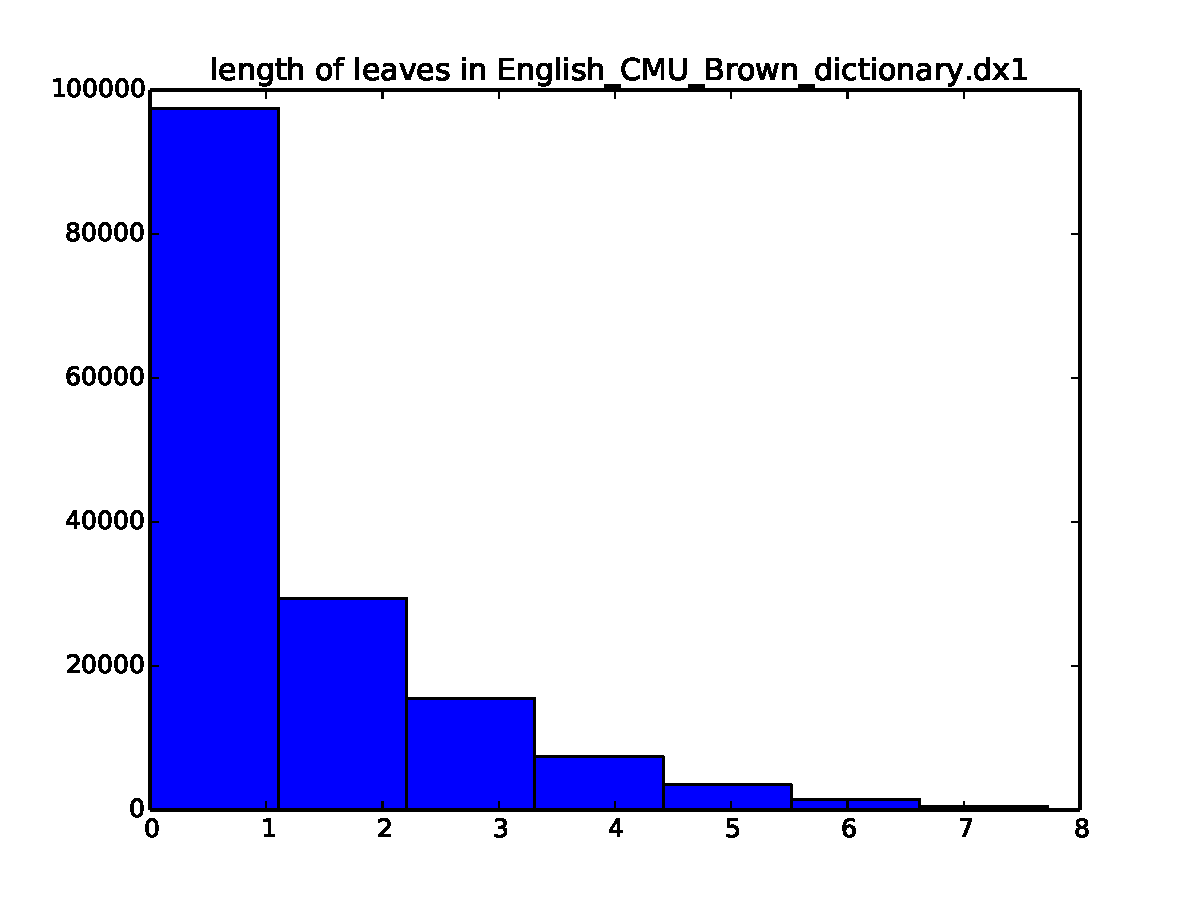
\includegraphics[scale=.5,page=1]{English_CMU_Brown_dictionary_dx1_histograms.pdf}
		\includegraphics[scale=.5,page=2]{English_CMU_Brown_dictionary_dx1_histograms.pdf}
		\includegraphics[scale=.5,page=3]{English_CMU_Brown_dictionary_dx1_histograms.pdf}
		\end{figure}
		
		\begin{figure}[H]
		\centering
		\caption{English 1k Corpus}
		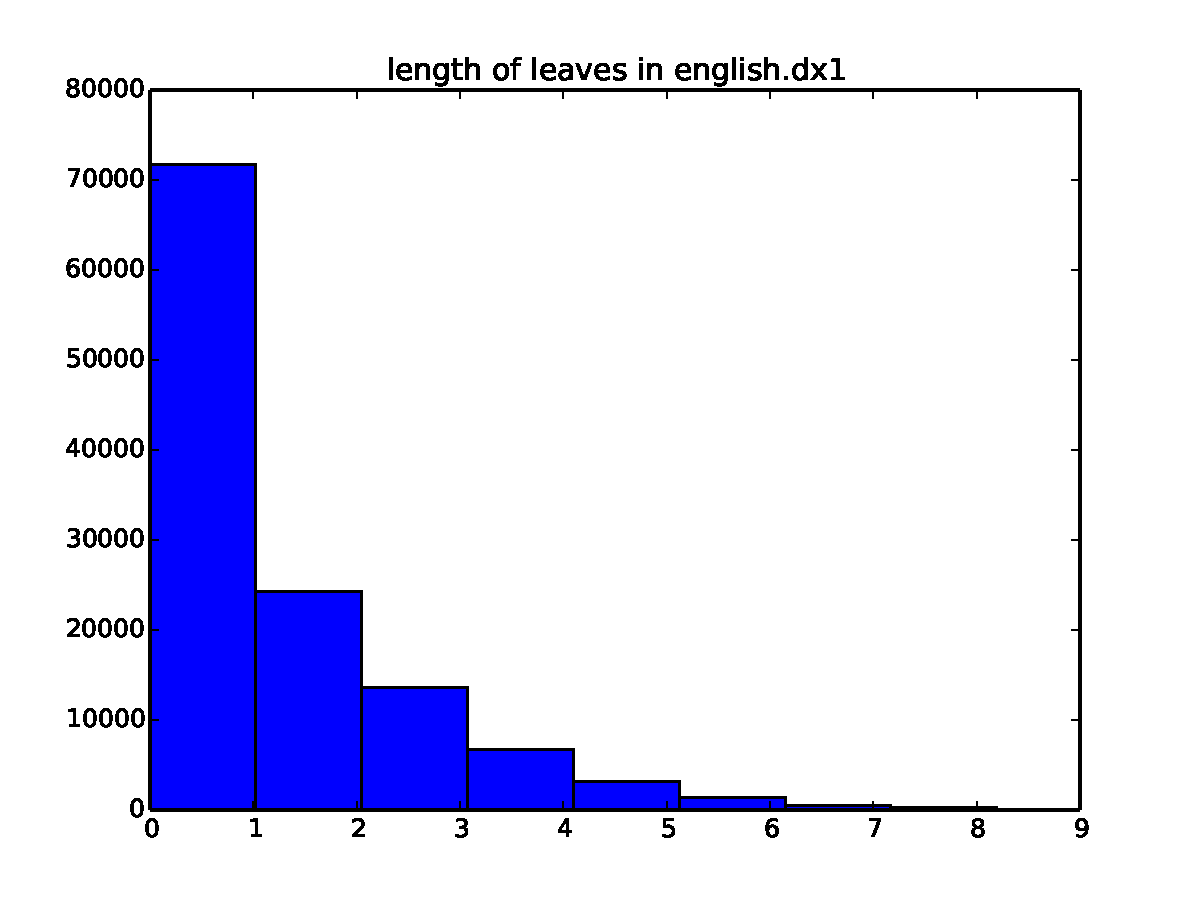
\includegraphics[scale=.5,page=1]{english_dx1_histograms.pdf}
		\includegraphics[scale=.5,page=2]{english_dx1_histograms.pdf}
		\includegraphics[scale=.5,page=3]{english_dx1_histograms.pdf}
		\end{figure}
		
We can see that they are similar as far as the distribution goes, but the values are not identical. This frustrates a numerical comparison, but the Quantile Quantile Plot resolves this by providing a visualization of a numerical similarity between unequal elements. Note that all QQplots feature the line y=x, and all analysis is done in the left to right direction. With more time, a right to left version could be easily developed.
		
		\begin{figure}[H]
		\centering
		\caption{Comparison of two English Corpuses}
		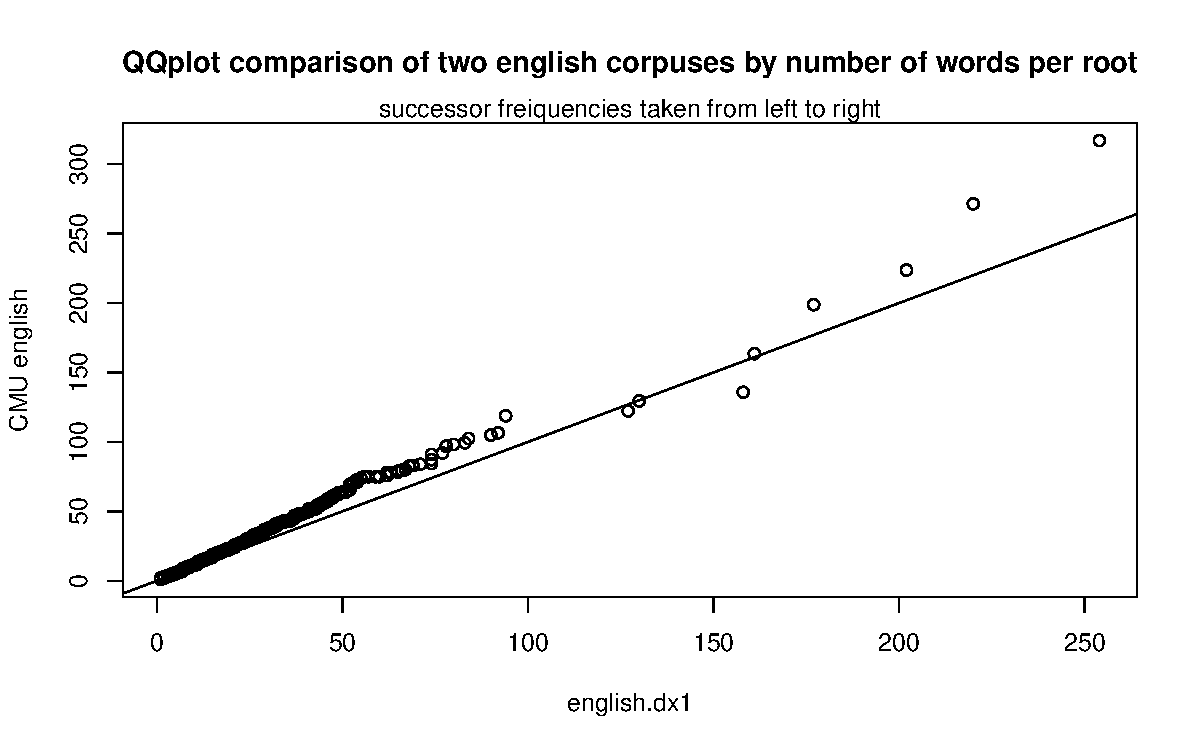
\includegraphics[scale=.7,page=1]{plots.pdf}
		\includegraphics[scale=.7,page=2]{plots.pdf}
		\end{figure}
		\begin{figure}[H]
		\includegraphics[scale=.7,page=3]{plots.pdf}
		\end{figure}
We see that although the data is a bit sparse, it follows the y=x trend fairly closely. 


Now we will look at a pair of known-similar language that share some features, where they diverge in others. These languages are Latin and Italian They are not mutually intelligible, but one develops directly from the other so their structure should be similar. 

		\begin{figure}[H]
		\centering
		\caption{Comparison of two Mediterranean Languages}
		\includegraphics[scale=.7,page=4]{plots.pdf}
		\end{figure}
		\begin{figure}[H]
		\centering
		\includegraphics[scale=.7,page=5]{plots.pdf}
		\includegraphics[scale=.7,page=6]{plots.pdf}
		\end{figure}
We see that a comparison of the length of chunks and chunks per word are very similar, perhaps meaning that the structure of the language is similar - prefixes are often 3 characters long, tense suffixes are 3 letters, superlative endings are 4 letters long, etc. However, on number of words per root diverge widely. This could be an indication of the increased grammatical complexity of latin, or it could be an indication on the larger more diverse vocabulary of Italian. 

In the full list of plots there are some interestingly similar languages - Catalan and French, for instance, are very similar despite their fierce political differences. 

To show that this method differentiates differing languages, we next compare Dutch and Finnish. A comparison of Dutch and Norwegian may yield similar plots, but Finnish, being closer to Russian (I think) and other Slavic languages rather than Germanic means that they diverge greatly. 

		\begin{figure}[H]
		\centering
		\caption{Comparison of Dutch and Finnish}
		\includegraphics[scale=.7,page=7]{plots.pdf}
		\includegraphics[scale=.7,page=8]{plots.pdf}
		\end{figure}
		\begin{figure}[H]
		\centering
		\includegraphics[scale=.7,page=9]{plots.pdf}
		\end{figure}

On no metic do Dutch and Finnish appear to be similar. We will now see if we can apply this method to the Voynich manuscript to determine its linguistic similarities.

%----------------------------------------------------------------------------------------
%	PROBLEM 2
%----------------------------------------------------------------------------------------

\section{Voynich}

The first thing to note is that there are several interpretations of the Voynich manuscript, and some are better than others. There was a very persistent problem with with majority of the interpretations not being long enough to draw any conclusions from, so I have only made plots for interpretations coded BTX, BFX, BF2, BC2, AL4, AF2, AF1, and AC1. The interpretations of these three letter codes in included in the problem description of homework 1. 

I made the most through comparison with BTX, and with the best language contenders I made further comparisons against other interpretations. Notably, I found BTX to be similar in some ways to English:

		\begin{figure}[H]
		\centering
		\caption{Comparison of BTX and English}
		\includegraphics[scale=.7,page=12]{plots.pdf}
		\end{figure}

This didn't hold up, however. They may be similar in length of chunks, but they differ greatly in words per root. As we saw in latin v italian, this may be indication of a common linguistic ancestor. With this on my mind I compared BTX to Modern German and was disappointed with their dissimilarity. 

		\begin{figure}[H]
		\centering
		\caption{Comparison of BTX and German}
		\includegraphics[scale=.7,page=17]{plots.pdf}
		\end{figure}

Modern Italian, too, seemed very dissimilar. 
		\begin{figure}[H]
		\centering
		\caption{Comparison of BTX and Italian}
		\includegraphics[scale=.7,page=19]{plots.pdf}
		\end{figure}
		
However, other interpretations were more favorable to italian, especially BFX:
		\begin{figure}[H]
		\centering
		\caption{Comparison of BFX and Italian}
		\includegraphics[scale=.7,page=22]{plots.pdf}
		\includegraphics[scale=.7,page=23]{plots.pdf}
		\end{figure}

Surprisingly, French also agreed with BFX:

		\begin{figure}[H]
		\centering
		\caption{Comparison of BFX and French}
		\includegraphics[scale=.7,page=25]{plots.pdf}
		\includegraphics[scale=.7,page=26]{plots.pdf}
		\end{figure}

In conclusion, if the metrics here are to be trusted, the linguistic origin of the Voynich manuscript appears to be northern Italy, some time between the fall or the roman empire and Italian Unification / the formation of Modern Italian. This is all corroborated by the geological evidence surrounding the Voynich Manuscript, so it is not exactly new information, but I did find it rather interesting! 

\end{document}